\begin{Ueberlieferung}% 
{\textit{L}}Aufzeichnung: LH XXXVII 5 Bl. 130. 1 Bl. 2\textsuperscript{o}. 1 S. auf Bl. 130~r\textsuperscript{o}. Bl. 130~v\textsuperscript{o} leer.\\%
Cc 2, Nr. 976
\end{Ueberlieferung}%
%
\begin{Datierungsgruende}%
Die inhaltliche Verwandtschaft mit dem Stück N. 15 
% 037_05_128-129 = De motu gravium naturali
lässt einen gemeinsamen Entstehungszeitraum vermuten, der hier für die Datierung übernommen wird.
\end{Datierungsgruende}
%
\count\Afootins=1000
\count\Bfootins=1000
\count\Cfootins=1200
%\pstartfirst
%[Bl. 130~r\textsuperscript{o}]
%% [130~r\textsuperscript{o}] 
%\pend
%\pstart \noindent
%\begin{window}[0,r,\hspace{4mm}\includegraphics[%trim = -3mm -2mm 0mm 0mm, clip,
%width=0.4\textwidth]
%{images/LH037,05_130r-d.pdf},\hspace{25mm} {[\textit{Fig. 1}]}]
%\noindent
%$\displaystyle a$ = tempus \edtext{quo}{\lemma{quo initium spatii}\Bfootnote{\textit{(1)}\ primum spatium \textit{(2)}\ initium spatii \textit{L}}} percurritur.
%\newline%
%$b.$ initium spatii.
%\newline%
%$\gamma.$ ratio spatii ad initium spatii.
%\newline%  
%$b\gamma.$ {spatium\reversemarginpar\marginnote{\scriptsize\hspace{-13mm}10}}.
%\newline%
%\rule[-4mm]{0mm}{10mm}% PR: Rein provisorisch !!!
%$\displaystyle\frac{ab\gamma}{2}.$ tempus quo spatium \edtext{percurritur.
%\newline%
%Initium}{\lemma{11f. \hspace{1.8mm} percurritur.}\killnumber\Bfootnote{\textit{(1)}\ $\theta$ ratio \textit{(2)}\ Initium \textit{L}}}
%temporis idem est cum tempore quo initium spatii percurritur
%\edtext{$a.$ Ratio}{\lemma{13\hspace{1.8mm}}\killnumber\Bfootnote{ $a.$ \textit{(1)}\ $\theta$ \textit{(2)}\ Ratio \textit{L}}} temporis totius ad initium temporis
%\rule[-4mm]{0mm}{10mm}% PR: Rein provisorisch !!!
%$=\displaystyle\frac{b\gamma}{2}$.
%%\vspace*{1.0em}%
%\newline%
%\indent%
%Si grave\protect\index{Sachverzeichnis}{grave} descendat \edtext{in tempore}{\lemma{15 \hspace{1.8mm} in}\killnumber\Bfootnote{\textit{(1)}\ linea \textit{(2)}\ tempore \textit{L}}} $ab$
%{secto\reversemarginpar\marginnote{\scriptsize\hspace{-13mm}15}}  in quotcunque partes aequales, ita ut, quolibet momento tantum impetus\protect\index{Sachverzeichnis}{impetus} \edtext{non}{\lemma{17 \hspace{1.8mm}}\killnumber\Bfootnote{non \textit{erg.} \textit{L}}} acquirere intelligatur, \edtext{quantum primo motus momento}{\lemma{\hspace{1.8mm}18 \hspace{1.8mm} quantum}\killnumber\Bfootnote{\textit{(1)}\ initio \textit{(2)}\ primo motus momento \textit{L}}} habebat \edtext{erunt}{\lemma{18-S. 142.1 erunt}\killnumber\Bfootnote{\textit{(1)}\ quolibet momento \textit{(2)}\ in quolibet  \textit{(a)} lineae  \textit{(b)} temporis $ab$  \textit{(aa)} puncto  \textit{(bb)} momento \textit{L}}} in 
%\end{window}
%  \begin{wrapfigure}[12]{l}{0.4\textwidth}                    
%            \vspace{-4mm}  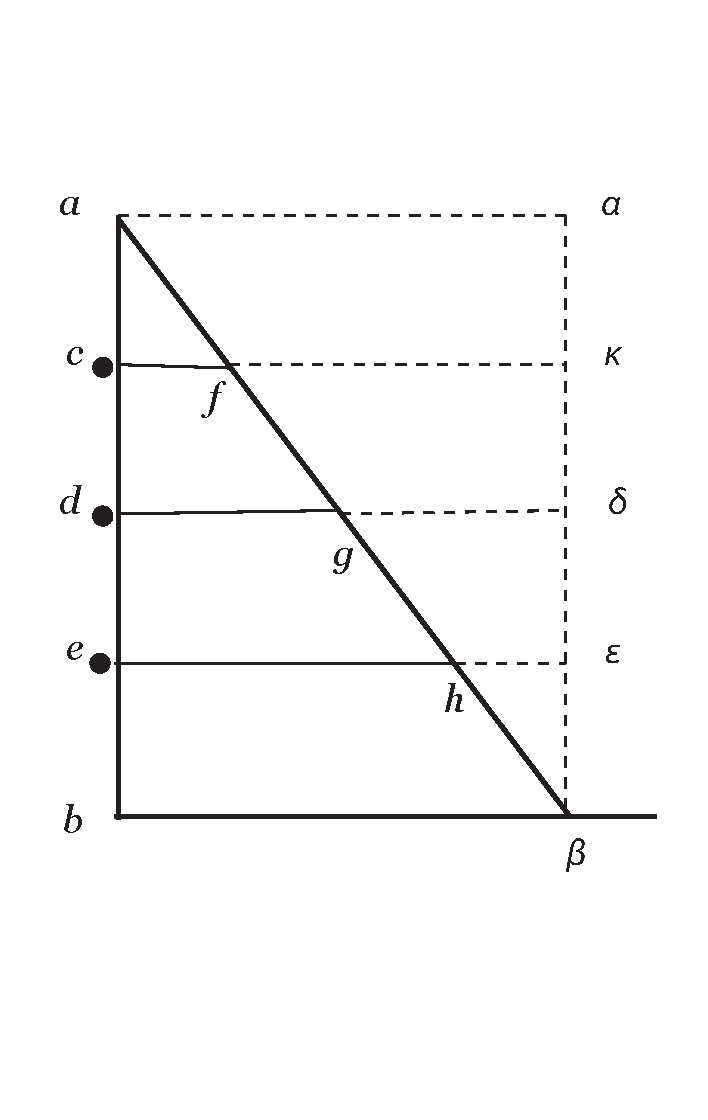
\includegraphics[trim = 0mm 0mm -3mm 0mm, clip, width=0.4\textwidth]{images/LH037,05_130r-d.pdf}\\
%              \noindent \centering [\textit{Fig. 1}]
%                \end{wrapfigure}
%\noindent%
%$\displaystyle a$ = tempus \edtext{quo}{\lemma{quo initium spatii}\Bfootnote{\textit{(1)}\ primum spatium \textit{(2)}\ initium spatii \textit{L}\ }} percurritur.
%\newline%
%$b.$ initium spatii.
%\newline%
%$\gamma.$ ratio spatii ad initium spatii.
%\newline%  
%$b\gamma.$ spatium.
%\newline%
%\rule[-4mm]{0mm}{10mm}% PR: Rein provisorisch !!!
%$\displaystyle\frac{ab\gamma}{2}.$ tempus quo spatium \edtext{percurritur.
%\newline%
%Initium}{\lemma{percurritur.}\Bfootnote{\textit{(1)}\ $\theta$ ratio \textit{(2)}\ Initium \textit{L }\ }}
%temporis idem est cum tempore quo initium spatii percurritur
%\edtext{$a.$ Ratio}{\lemma{$a.$}\Bfootnote{\textit{(1)}\ $\theta$ \textit{(2)}\ Ratio \textit{L}\ }} temporis totius ad initium temporis
%\rule[-4mm]{0mm}{10mm}% PR: Rein provisorisch !!!
%$=\displaystyle\frac{b\gamma}{2}$.
%%\vspace*{1.0em}%
%\newline%
%\indent%
%Si grave\protect\index{Sachverzeichnis}{grave} descendat \edtext{in tempore}{\lemma{in}\Bfootnote{\textit{(1)}\ linea \textit{(2)}\ tempore \textit{L}\ }} $ab$
%secto in quotcunque partes aequales, ita ut, quolibet momento tantum impetus\protect\index{Sachverzeichnis}{impetus} \edtext{non}{\lemma{}\Bfootnote{non \textit{erg.} \textit{L}}} acquirere intelligatur, \edtext{quantum primo motus momento}{\lemma{quantum}\Bfootnote{\textit{(1)}\ initio \textit{(2)}\ primo motus momento \textit{L}\ }} habebat \edtext{erunt}{\lemma{18-S. 142.1 erunt}\killnumber\Bfootnote{\textit{(1)}\ quolibet momento \textit{(2)}\ in quolibet  \textit{(a)} lineae  \textit{(b)} temporis $ab$  \textit{(aa)} puncto  \textit{(bb)} momento \textit{L}\ }} in 
\pstartfirst
[130~r\textsuperscript{o}]
\pend
\pstart\noindent
\begin{window}[0,r,\hspace{4mm}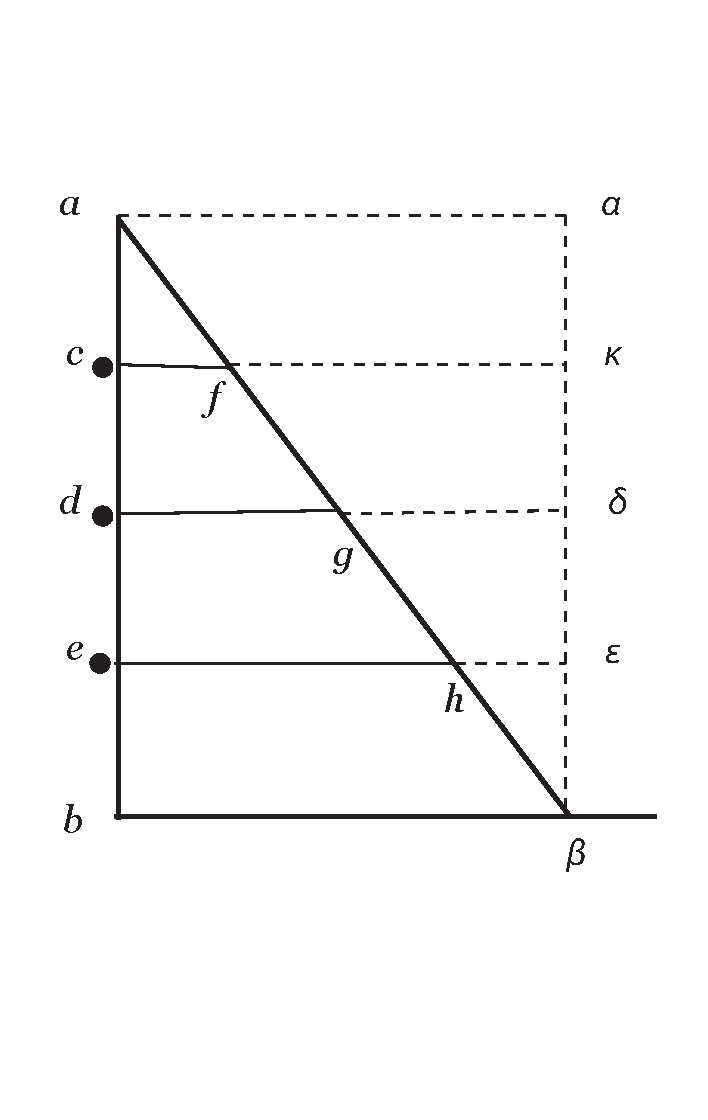
\includegraphics[% trim = -3mm -2mm 0mm 0mm, clip,
width=0.39\textwidth]
{images/LH037,05_130r-d.pdf},%
\hspace{24mm}{[\textit{Fig. 1}]}]
\noindent
$\displaystyle a$ = tempus \edtext{quo initium spatii}{\lemma{quo}\Bfootnote{\textit{(1)}\ primum spatium \textit{(2)}\ initium spatii \textit{L}}} percurritur.
\newline%
$b.$ initium spatii.
\newline%
$\gamma.$ ratio spatii ad initium spatii.
\newline%  
$b\gamma.$ {spatium\reversemarginpar\marginnote{\scriptsize\hspace{-13mm}10}}.
\newline%
\rule[-4mm]{0mm}{10mm}% PR: Rein provisorisch !!!
$\displaystyle\frac{ab\gamma}{2}.$ tempus quo spatium \edtext{percurritur.
\newline%
Initium}{\lemma{11f.\hspace{1.8mm}percurritur.}\killnumber\Bfootnote{\textit{(1)}\ $\theta$ ratio \textit{(2)}\ Initium \textit{L}}}
temporis idem est cum tempore quo initium spatii
\edtext{percurritur $a.$ Ratio}{\lemma{\hspace{1.8mm}13\hspace{1.8mm}percurritur $a.$}\killnumber\Bfootnote{\textit{(1)}\ $\theta$ \textit{(2)}\ Ratio \textit{L}}}
temporis totius ad initium temporis
\rule[-4mm]{0mm}{10mm}% PR: Rein provisorisch !!!
$=\displaystyle\frac{b\gamma}{2}$.
\newline\noindent%
Si grave\protect\index{Sachverzeichnis}{grave}
\edtext{descendat in tempore}{\lemma{15\hspace{1.8mm}descendat in}\killnumber\Bfootnote{\textit{(1)}\ linea \textit{(2)}\ tempore \textit{L}}} $ab$
{secto\reversemarginpar\marginnote{\scriptsize\hspace{-13mm}15}} in quotcunque partes aequales, ita ut, quolibet momento tantum impetus\protect\index{Sachverzeichnis}{impetus}
\edtext{novi}{\lemma{17\hspace{1.8mm}novi}\killnumber\Bfootnote{\textit{erg. L}}}
acquirere intelligatur,
\edtext{quantum primo motus momento}{\lemma{\hspace{1.8mm}17f.\hspace{1.8mm}quantum}\killnumber\Bfootnote{\textit{(1)}\ initio \textit{(2)}\ primo motus momento \textit{L}}}
habebat, \edtext{erunt }{\lemma{\hspace{1.8mm}18f.\hspace{1.8mm}erunt}\killnumber\Bfootnote{%
\textit{(1)}\ quolibet momento \textit{(2)}\ in quolibet  \textit{(a)} lineae  \textit{(b)} temporis $ab$  \textit{(aa)} puncto  \textit{(bb)} momento \textit{L}}}
in quolibet%
\end{window}
\pend
%\newpage
\pstart%
\noindent%
temporis\setline{19} $ab$ momento\edlabel{37,05_130r_xy2}
ut $c.$ $d.$ $e.$ $b.$ impetus,\protect\index{Sachverzeichnis}{impetus}
ut altitudines, seu impetus
\edtext{vel percussio,\protect\index{Sachverzeichnis}{percussio}}{\lemma{vel percussio}\Bfootnote{\textit{erg. L}}}
in puncto $c$ ad impetum vel percussionem in puncto $d$ erit ut $AC$ ad $AD.$
Ergo impetus poterunt
\edtext{exprimi rectis}{\lemma{exprimi}\Bfootnote{\textit{(1)}\ lineis \textit{(2)}\ rectis \textit{L}}}
parallelis ad altitudines proportionalibus $cf$. $dg$. $eg$. $be$. aliisque intermediis, omnium
\edtext{impetuum}{\lemma{impetuum}\Bfootnote{\textit{erg. L}}}
aggregatum durante descensu ex $A$ in $C$ comparari poterit Triangulo $ACF$ et ex $A$ in $B$ Triangulo $AB\beta.$
Cum autem velocitates sunt aggregata impetuum ut motus conatuum,
(:~est enim \protect\index{Sachverzeichnis}{velocitas}velocitas, \protect\index{Sachverzeichnis}{quantitas motus}quantitas
\edtext{motus, ut impetus\protect\index{Sachverzeichnis}{impetus} quantitas conatus\protect\index{Sachverzeichnis}{quantitas conatus}}%
{\lemma{motus, ut}\Bfootnote{%
\textit{(1)}\ aestimatio conatus %
\textit{(2)}\ quantitas conatus \textit{L}}}~:)
erunt velocitates, et per consequens spatia decursa temporibus, inde ab initio motus assumtis, ut $AC$ vel $AD.$ ut temporum
\edtext{quadrata. Et spatia}{\lemma{quadrata.}\Bfootnote{%
\textit{(1)}\ Et tempo %
\textit{(2)}\ Unde si spatia %
\textit{(3)}\ Et spatia \textit{L}}}
temporibus aequalibus decursa, crescent ut numeri
\edtext{impares}{\lemma{impares}\Bfootnote{\textit{erg. L}}}
deinceps ab unitate.
Ergo si tempore $AC$ percurratur pes unus tempore $CD,$
percurrentur 3. tempore $DE.$ 5. tempore $EB.$ 7. etc.
Et si tempore $AC$ percurretur pes unus, tempore $AD$
\edtext{percurrentur 4. tempore}{\lemma{percurrentur 4.}\Bfootnote{\textbar\ et \textit{gestr.} \textbar\ tempore \textit{L}}}
$AE.$ 9. tempore $AB.$ 16.
\pend
\pstart
\edtext{Hactenus tempore metiti sumus accelerationem,\protect\index{Sachverzeichnis}{acceleratio}}{\lemma{Hactenus}\Bfootnote{%
\textit{(1)}\ rem a tem %
\textit{(2)}\ tempore [...] accelerationem, \textit{L}}}
nunc videamus, an et spatio eam metiri liceat, ut veteribus, et nostro tempore philosophis quibusdam placuit.
Esto spatium percurrendum $\alpha\beta$, in
\edtext{quo motus gravis\protect\index{Sachverzeichnis}{grave}}{\lemma{quo}\Bfootnote{%
\textit{(1)}\ grave %
\textit{(2)}\ motus gravis \textit{L}}}
descendentis, ita acceleretur si fieri potest, ut in quolibet novo spatii puncto
\edtext{$\kappa.$ $\delta.$ $\epsilon.$ $\beta$ impetum}{\lemma{$\kappa.$ $\delta.$ $\epsilon.$ $\beta$}\Bfootnote{%
\textit{(1)}\ momentum %
\textit{(2)}\ impetum \textit{L}}}
acquirat primo parem.
Quare ut \edtext{ante recta}{\lemma{ante}\Bfootnote{%
\textit{(1)}\ linea %
\textit{(2)}\ recta \textit{L}}}
$AB$ \edtext{tempora, rectis}{\lemma{tempora,}\Bfootnote{%
\textit{(1)}\ lineis %
\textit{(2)}\ rectis \textit{L}}}
$CF.$ $DG.$ $EH.$ $B\beta$ etc. eorumque aggregatis spatia metiti sumus;
ita contra cum recta $\alpha\beta$ nunc
\edtext{spatium complectamur,}{\lemma{spatium}\Bfootnote{%
\textit{(1)}\ metiamur, %
\textit{(2)}\ complectamur, \textit{L}}}
rectis $A\alpha$. $C\kappa$ etc. et parallelis
\edtext{tempora exprimemus.}{\lemma{tempora}\Bfootnote{%
\textbar\ seu impetus \textit{erg. u. gestr.} \textbar\ exprimemus \textit{L}}}
Cumque crescente impetu\protect\index{Sachverzeichnis}{impetus} ut ante spatia creverunt,
ita \edtext{nunc tempora decrescant, tempora}{\lemma{nunc tempora}\Bfootnote{%
\textbar\ vel impetus \textit{erg. u. gestr.} \textbar\ decrescant, %
\textit{(1)}\ erit %
\textit{(2)}\ hab %
\textit{(3)}\ tempora \textit{L}}}
continebuntur Triangulo inverso $A\alpha\beta$. Et tempora
\edtext{quibus aequalia spatia percurruntur }{\lemma{quibus [...] percurruntur}\Bfootnote{\textit{erg. L}}}
nempe trapezia $\textit{Af}\kappa\alpha$. $\textit{fg}\delta\kappa$ etc. erunt ut numeri impares retrogradi versus unitatem.
Et si spatium $\alpha\kappa$ decurretur tempore ut 7. spatium $\kappa\delta$ decurretur tempore ut 5.
spatium $\delta\epsilon$ tempore ut 3. spatium $\epsilon\beta$ tempore ut 1.
\pend 
\pstart
Ex his apparet nullam esse rationem,
\edtext{cur altera Hypothesium}{\lemma{cur}\Bfootnote{%
\textit{(1)}\ alia Hypothesis %
\textit{(2)}\ altera Hypothesium \textit{L}}}
alteri praeferri debeat, cum altera alterius inversa sit, modo tempora spatiis
\edtext{substituantur: ergo}{\lemma{substituantur:}\Bfootnote{%
\textit{(1)}\ illud tam %
\textit{(2)}\ ergo \textit{L}}}
necesse est, aut neutram esse veram, aut coincidere
utramque.%
\edtext{}{\lemma{}\Afootnote{\textit{Im Anschluss:} Falsum.}}
\pend
\count\Afootins=1500
\count\Bfootins=1500
\count\Cfootins=1500

